%\addcontentsline{toc}{chapter}{Development Process}
\chapter{Design}

\section{Overall Architecture}

\subsection{Class Descriptions}
\subsubsection{Game Classes}
The game class section will describe the different classes used within the project and where they link with the use of diagrams to help illastrate.
\begin{figure}[h]
\centering
\label{fig:Game_Classes}
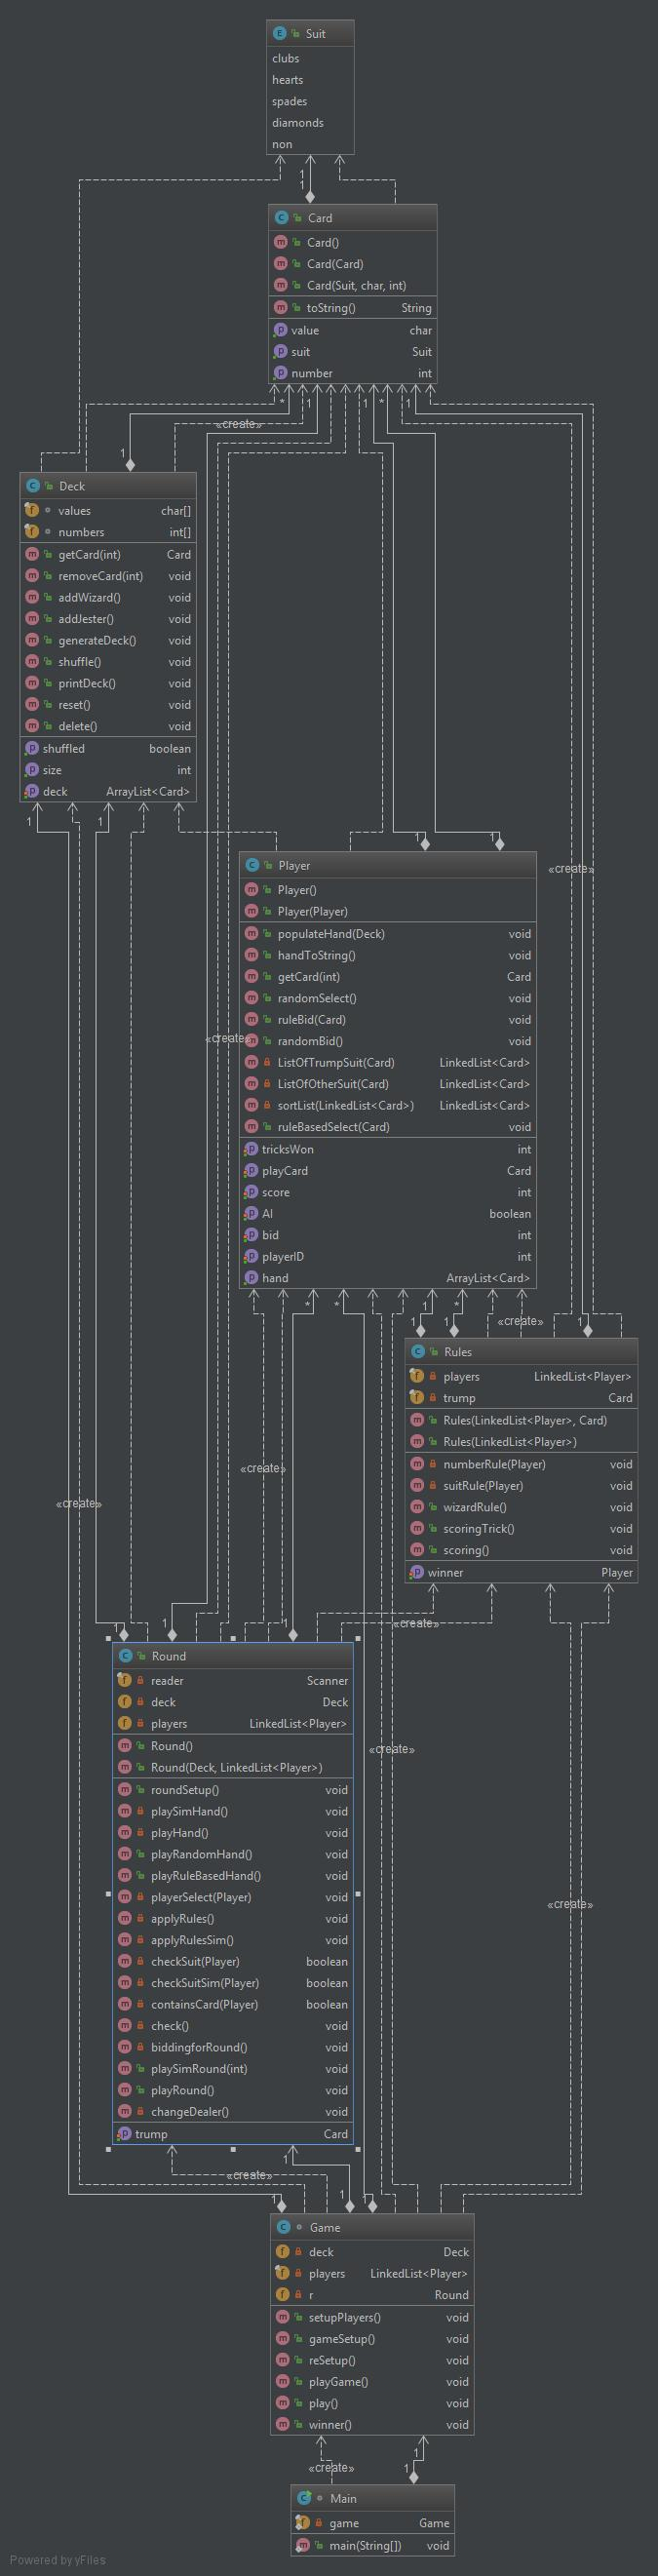
\includegraphics[width=15cm ,height=20cm,keepaspectratio]{Game_Classes}
\caption{Diagram Showing the Class Diagram of the Game Classes}
\end{figure}
\paragraph{Card}
This Card class created Card objects that will contain variables for the suit, the value of the card in relation to the other and the number displayed on the card such as a wizard or an ace. It will also contain methods to construct the card and getters and setters for each of the variables. Card will also contain a copying constructor for the use of the AI. This class will mainly be used in the generation of the deck but will also be used in the in other methods to refer to the suit and number(the value of the card in reference to the game, like ace being worth 14) used within the cards
\paragraph{Deck}
Deck is a class for create a deck object to be used for in the classes of game, round and the Monte Carlo Tree Search. It contains variables for an array of cards, and array of the different values there are for the cards and the numbers they each will have. There is also a Boolean variable to check if the deck has been shuffled. The deck class will also contain values to create and the wizards and jester cards to be added to the normal 52 card deck that is generated with a different method. there will also be a method to shuffle the deck of cards so that each player gets different cards for each round.
\paragraph{Player} 
The player class constructs the player objects that will contains variable for the player id; the cards they currently have in there hand; there bid and score; the card they have played for the trick; how many trick they have won and if it is an AI or normal player. This class will contain the getters and setts for the these variable whenever they will be need. It will also contain methods to print out the hand they currently have; constructors to copy the players variables; to populate the hand of the deck from cards they are within the deck. the is methods to randomly and rule based selection the cards and bids for the more simple AI.
\paragraph{Round}
the Round class wi
\paragraph{Rules}
\paragraph{Game}
The game class contains methods to setup up the game with variables for the array of 3 players and how many are human, the round  and the deck used. This class also contains methods to resetup the game, how many rounds are players and who the winner of the game is.
\paragraph{Suit}
An enumerator class that contains the 5 different suits that the card could be such as heart, spades, clubs, diamonds and non for the wizard and jester cards.
\paragraph{Main}
This it the main class used to intailise the game and contains the game object for this to happen.
\subsubsection{Aritifical Intelligence Classes}
\begin{figure}[h]
\centering
\label{fig:AI_Classes}
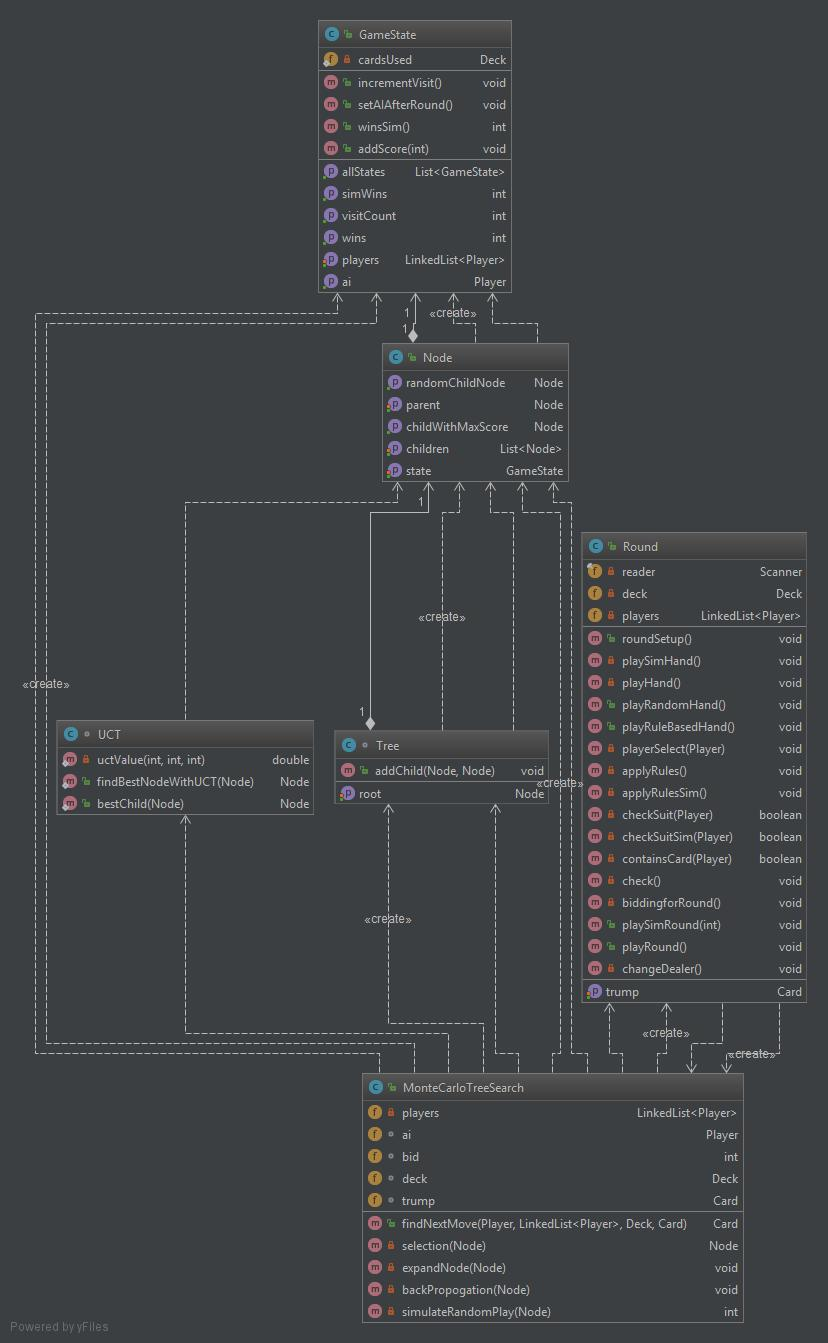
\includegraphics[width=15cm ,height=20cm,keepaspectratio]{AI_Classes}
\caption{Diagram Showing the Class Diagram of the AI Classes and the linking Round Class}
\end{figure}
This section will show you the classes associated with Monte Carlo Tree Search AI it made more sense for the complex Ai to be separate from the main game.
\paragraph{Node}

\paragraph{Tree}
\paragraph{GameState}
\paragraph{MonteCarloTreeSearch}
\paragraph{UCT}

\subsection{Data Flow Diagrams}
\section{Some detailed design}
In this section I will outline the important Algorithms to be used in the program and discuss how the User interface will looked and function.
\subsection{Algorithm Design}
\subsubsection{Scoring}
\begin{figure}
\centering
\label{fig:Scoring}
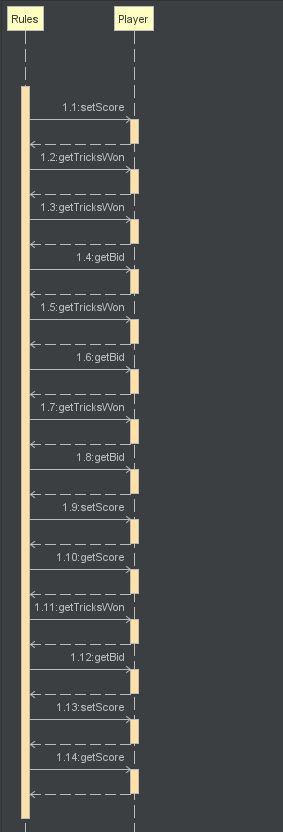
\includegraphics[width=15cm ,height=20cm,keepaspectratio]{ScoringSequenceDiagram}
\caption{Sequence Diagram of Scoring Method for Algorithm Description}
\end{figure}
\subsubsection{WinSim}
\begin{figure}
\centering
\label{fig:WinSim}
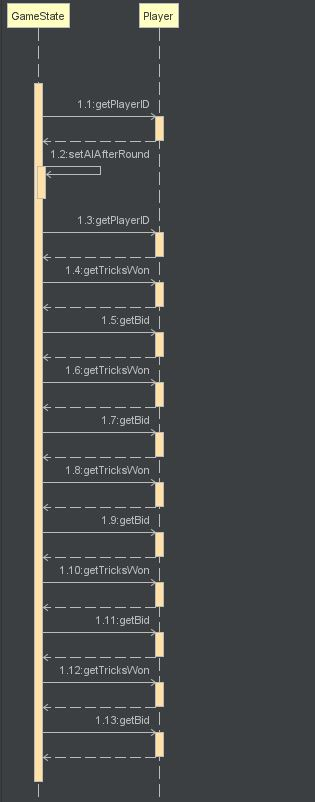
\includegraphics[width=15cm ,height=20cm,keepaspectratio]{WinSimSequenceDiagram}
\caption{Sequence Diagram of WinSim Method of Winning simulation Algorithm }
\end{figure}
\subsubsection{Rules}
\begin{figure}
\centering
\label{fig:Rules}
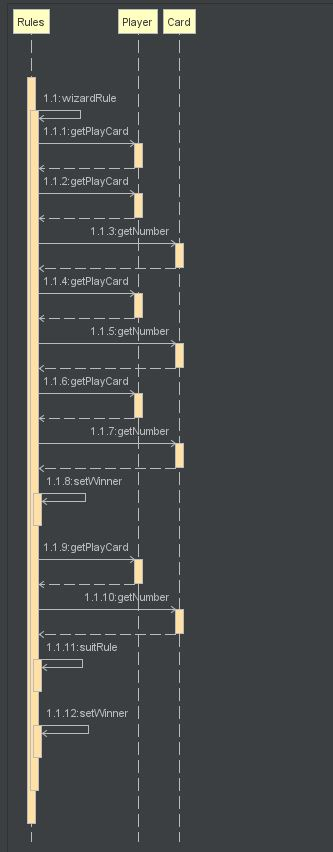
\includegraphics[width=15cm ,height=20cm,keepaspectratio]{RuleSequenceDiagram}
\caption{Sequence Diagram for the Rules Algorithm}
\end{figure}
\subsubsection{Play Hand}
\begin{figure}
\centering
\label{fig:Play}
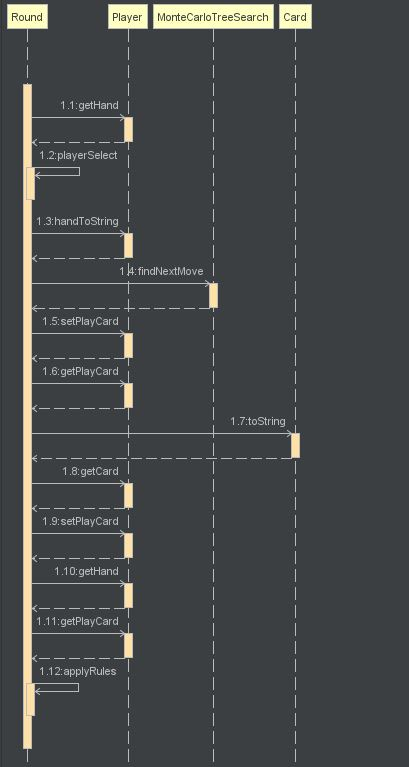
\includegraphics[width=15cm ,height=20cm,keepaspectratio]{PlayHandSequenceDiagram}
\caption{Sequence Diagram of Play Hand method for the Algorithm that shows what happens when a card is played}
\end{figure}
\section{User Interface}
As this project is mainly based on the Artificial Intelligence, only a simple User interface is needed. So, using a Terminal UI seems the best choice. This will include showing the cards that the player has in their hand and the card they will play. This interface will also allow you to bid at the beginning of the round after the trump card and hands have been given out. After the round has been completed it shows the number of tricks that has been won, the score they have received based on their bid and trick they have won.



